In diesem Versuch wird die optische Pinzette kennengelernt. Es handelt sich dabei um einen Laser, mit dessen Hilfe kleine Objekte wie Mikroorganismen bewegt werden können. Diese Technik wird beispielsweise bei der In-Vitro-Fertilisation angewandt.

\section{Funktionsweise der optischen Pinzette}

\subsection{Geometrische Optik}
\label{sec:gradient}
Im Rahmen der geometrischen Optik betrachtet man Licht als Strahlen, deren Welleneigenschaften vernachlässigt werden. Diese Näherung ist sinnvoll, solange die Dimensionen der Objekte mit denen das Licht wechselwirkt groß gegen die Wellenlänge sind.
Ein Lichtstrahl besitzt dabei einen Impuls in Strahlrichtung, der proportional zur Intensität ist. Betrachte nun einen Lichtstrahl, der auf eine dielektrische Sphäre trifft \cite{Ashkin}: 
Der Lichtstrahl wird gebrochen, und ändert somit seine Richtung. Dabei überträgt er einen Impuls auf die Kugel. Treffen nun zwei Lichtstrahlen  unterschiedlicher Intensität auf die Kugel (s. Abb. \ref{fig:geom_optik}), so zeigt die resultierende Kraft in Richtung des Lichtstrahls mit der höheren Intensität.
Ein Laser besitzt ein gaussförmiges Intensitätsprofil, das in der Mitte ein Maximum besitzt. Trifft also ein Laserstrahl auf eine dielektrische Kugel, so wirkt eine rückstellende Kraft in Richtung der Strahlmitte. Die Kugel ist also ``gefangen''.

\begin{figure}[h]
	\centering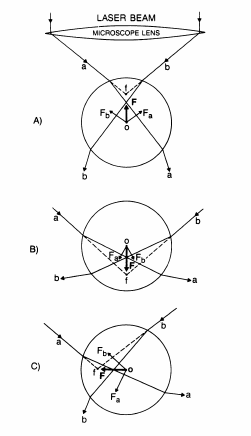
\includegraphics[width=0.5\textwidth]{fig/geom_optik.png}
	\caption{Skizze von Lichtstrahlen, die auf dielektrische Kugeln treffen \cite{Ashkin}}
	\label{fig:geom_optik}
\end{figure}

\subsection{Wellenoptik}

Ist die Größe des Objekts im Bereich der Wellenlänge des Lichts, so muss die maxwellsche Elektrodynamik zur Beschreibung des Phänomens verwendet werden. Das elektromagnetische Feld induziert im Objekt ein Dipolmoment $\vec{P}$. Die Wechselwirkungsenergie mit dem Feld ist dann gegeben durch
\begin{equation}
 V = -\vec{P}\cdot\vec{E}.
\end{equation}
Da gilt
\begin{equation}
 \vec{P} \propto \vec{E},
\end{equation}
folgt daraus mit $I\propto\vec{E}^{2}$
\begin{equation}
 V \propto -I.
\end{equation}
Das Potentialminimum befindet sich also an der Stelle der höchsten Intensität.

\section{Brownsche Bewegung}

Bei der Brownschen Bewegung handelt es sich um die zufällige Bewegung von kleinen Teilchen in einer Flüssigkeit. Diese besitzen nämlich eine mittlere kinetische Energie von 
\begin{equation}
 <E_{kin}> = \frac{f}{2}k_{\textrm{B}}T,
\end{equation}
mit der Temperatur $T$ und der Anzahl der Freiheitsgrade $f$. Die beobachtete ``Zitterbewegung'' kommt dadurch zustande, dass die Teilchen ständig miteinander stoßen.

Das mittlere Abstandsquadrat eines Teilchens ist \cite{Litmap}
\begin{equation}
 <r^{2}>(t) = \frac{1}{n}\sum_{i}^{n}r^{2}(t_{i}).
\end{equation}
In der Flüssigkeit sind die Teilchen Stokesscher Reibung ausgesetzt
\begin{equation}
 F_{\textrm{R}} = 6\pi\eta_{eff}av,
\end{equation}
mit der effektiven Viskosität der Flüssigkeit $\eta_{eff}$, dem Radius der Teilchen $a$ und ihrer Geschwindigkeit $v$. Es ergibt sich
\begin{equation}
 <r^{2}>(t) = 4Dt,
\end{equation}
mit dem Diffusionskoeffizienten
\begin{equation}
 D = \frac{k_{\textrm{B}}T}{6\pi\eta_{eff}a}.
\end{equation}

Da die Brownsche Bewegung ein statistisches Phänomen ist, kann die Bewegung eines Teilchens mit Hilfe einer Wahrscheinlichkeitsverteilung beschrieben werden. Die Aufenthaltswahrscheinlichkeit bei Anwesenheit eines Potentials $U$ ist gegeben durch \cite{Litmap}
\begin{equation}
 P(x) = \frac{1}{Z}\exp\left(-\frac{U(x)}{k_{\textrm{B}}T}\right),
\end{equation}
wobei $Z$ einen Normierungsfaktor bezeichnet.

\subsection{Maximale Fangkraft}

Die maximale Fangkraft $F_{\textrm{T}}$ des Lasers kann durch Messung der maximalen Geschwindigkeit, mit der die Kugeln bewegt werden können, bestimmt werden. Im Grenzfall gilt
\begin{equation}
 F_{\textrm{T}} = F_{\textrm{R}} = 6\pi\eta_{eff}av_{\textrm{max}}.
\end{equation}
Dies kann mit Hilfe des Diffusionskoeffizienten ausgedrückt werden
\begin{equation}
 F_{\textrm{T}} = \frac{k_{\textrm{B}}T}{D} v_{\textrm{max}}.
\end{equation}




